% Physics in the Household

\documentclass[11pt]{article}

\usepackage[a4paper, margin=1in]{geometry}

\usepackage{amsmath}

\usepackage{amssymb}

\usepackage[german]{babel}

\usepackage[autostyle=true]{csquotes}

\usepackage{libertine}

\usepackage[libertine]{newtxmath}

\usepackage{tikz}

\usepackage{gensymb}

\usepackage{fancyhdr}

\usepackage{amsfonts}

\usepackage{pgfplots}

\pgfplotsset{compat=1.10}

\usepackage{multicol}

\usepackage{caption}

\usepackage{floatrow}

\everymath{\displaystyle}

% Header / footer settings

\pagestyle{fancy}
\fancyhf{}
\renewcommand{\headrulewidth}{0.2mm}
\fancyhead[C]{Funktionen}
\renewcommand{\footrulewidth}{0.2mm}
\fancyfoot[L]{Peter Goldsborough}
\fancyfoot[C]{\thepage}
\fancyfoot[R]{\today}

\fancypagestyle{plain}{%
	\fancyhf{}
	\renewcommand{\headrulewidth}{0mm}%
	\renewcommand{\footrulewidth}{0.2mm}%
	\fancyfoot[L]{Peter Goldsborough}
	\fancyfoot[C]{\thepage}
	\fancyfoot[R]{\today}
}


\setlength{\headheight}{15pt}

\setlength{\parindent}{0pt}

\addtolength{\parskip}{\baselineskip}


\newcommand{\overbar}[1]{\mkern 1.5mu\overline{\mkern-1.5mu#1\mkern-1.5mu}\mkern 1.5mu}

\newcommand{\heading}[1]{\begin{center}\Huge \textbf{#1}\end{center}\par}

\newcommand{\sub}[1]{\vspace{\parskip}{\LARGE\textbf{#1}}}

\newcommand{\subsub}[1]{{\Large \textbf{#1}}}

\newcommand{\subsubsub}[1]{\textbf{#1}}

\newcommand{\colvec}[1]{\begin{pmatrix}#1\end{pmatrix}}

\newcommand{\extrapar}{\par\vspace{\baselineskip}}

\newcommand{\zitat}[1]{\foreignquote{german}{#1}}

\newcommand{\bolditem}[1]{\item \textbf{#1}}

\newcommand{\titleitem}[1]{\bolditem{#1}\par}

\newcommand{\defas}{ \dots \,\,}

\begin{document}
\thispagestyle{plain}

\heading{Physics in the Household}

\sub{Electrical Safety Precautions}

\subsub{Wires}

Power supplies carrying current to and from household appliances commonly consist of three wires: a \emph{live} wire, a \emph{neutral} wire and an \emph{earthing} wire. Current flows from the mains through the live wire to the appliance, and flows back to the mains through the neutral wire. The earthing wire (usually colored green or yellow), provides a low resistance path to ground (earth). This earthing wire is usually connected to (touches) the casing of the appliance such that, were a fault to occur and current from the live wire somehow be able to flow through the case, it would be directed to earth safely without causing any harm to the user. This is especially important when the case is made of a conductive material such as metal, while it is needed less for plastic covers. Consider the situation of a hairdryer being used in a moist or wet environment such as a bathroom. It may occur that some water happens to provide a conductive path between the current flowing through the live wire and the casing of the hairdryer, which moreover may be made of a metallic material. Were there no earthing wire to provide a low-resistance path for the current to flow to ground, the current would flow through the next-best path to ground: the person using the hairdryer. The result is that the person receives an electrical shock. This is why the earthing is a highly important component of any appliance's wiring. 

To ensure that electric current flows through a wire as safely as possible, minimizing the possible damage to humans handling the wires, all wires are \emph{insulated}. In fact, there are two layers of insulation: \emph{functional} insulation and \emph{protective} insulation. Each of the three wires described above, the neutral, live and earthing wire, is insulated individually to prevent the copper wires from touching (which may lead to a short circuit). The second, outer layer of insulation --- the \emph{protective} insulation --- solely protects the wires from outside influences. 

\begin{plot}
	
	% Protective insulation
	\draw [very thick, orange] (0, 0) circle [radius=1cm];

	% Protective insulation label
	\draw [<-, orange]
	      (0, -1.1) -- ++(0, -1) node [below] {Protective insulation};

	% Live wire
	\draw [fill=brown, very thick] (-0.45, -0.3) circle [radius=0.4];

	% Live wire label
	\draw [<-] (-0.45, -0.3) -- ++(-1, 0) node [left] {Live Wire};

	% Neutral wire
	\draw [fill=cyan, very thick] (0.45, -0.3) circle [radius=0.4];

	% Neutral wire label
	\draw [<-] (0.45, -0.3) -- ++(1, 0) node [right] {Neutral Wire};

	% Earthing wire
	\draw [fill=green, very thick] (0, 0.5) circle [radius=0.4];

	% Earthing wire label
	\draw [<-] (0, 0.5) -- ++(0, 1) node [above] {Earthing Wire};

	% Functional isolation label
	\draw [red, ->] (-3, 1) node [above] {Functional Isolation} -- (-0.8, 0);

\end{plot}

\sub{Fuses}

Fuses are thin pieces of metal that are added to power supplies and in other areas within a household, that open a circuit in case of a short circuit or current overload (e.g. from too many devices drawing too much current from a power supply). The working principle of such fuses is simply that they melt when the current strength is too high, typically around 20 Amperes. Thus, you should check the fuses of your electricity box if your oven or stove suddenly goes out. It and all other appliances connected to the same power outlet may have been drawing too much current.

\sub{Residual Current Circuit Brakers}

A Residual Current Circuit Braker (RCCB) is an electrical device typically found in your home's electricity box, that is used to interrupt an electric circuit in case of a fault in an appliance or due to any other current leakage (such as when current from the live wires flows to ground through a human instead of the neutral wire).

\begin{figure}[h!]
	\centering
	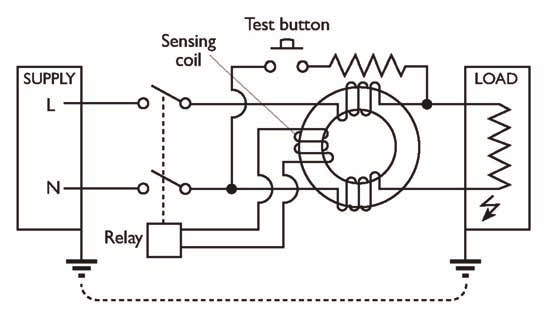
\includegraphics[scale=0.7]{img/rccb}
\end{figure}

Under normal conditions, the alternating current flowing through the live wire towards the load generates an alternating magnetic field around and within the first coil wrapped around the soft iron ring. This alternating magnetic field causes the magnetic flux within the soft iron ring to change with time and would, if this were the end of the story, induce an alternating voltage within the \emph{sensing coil}. However, if all goes well and there is no fault and current leakage in the load, the same alternating current from the live wire also flows through the neutral wire with the same strength and thus through the secondary coil on the lower end of the soft iron ring. This secondary coil has the same number of turns and is wound in the same way as the primary coil, such that the magnetic field generated in the secondary coil will equal the magnetic field produced in the first in terms of strength and magnitude, but will be phase shifted 180\degree{} or $\pi$ radians due to the way they are wound (in the same way). As a result, under normal conditions, the magnetic field will phase cancel and thus there will be no change in magnetic flux to induce a voltage in the sensing coil. 

However, if there is a fault in the appliance to which the live and neutral wire are connected, some or all of the current may not end up flowing back through the neutral wire, but to ground via a human or some other path. Consequently, the current flowing through the neutral wire will be less than the original current that was drawn from the load through the live wire and, as a result, the magnetic field produced in the secondary coil on the side of the neutral wire will not equal the magnetic field from the live wire. There will thus be a certain changing magnetic flux experienced by the sensing coil, such that a voltage is induced. This will cause an induced current to flow through the relay, which opens the connections of the live and neutral wire. Thus, the circuit would be broken and no more current would flow to ground in any way that it normally shouldn't. This happens very quickly, as RCCBs typically react within milliseconds and detect current strength differences as small as 10 milli-amperes. 

To test if the RCCB is working, the test button may be used. The resistance in the test circuit is lower than the resistance of the load, such that the charges flowing will prefer the path of less resistance and flow through the test circuit and not to the load. However, the alternating current will already have generated an alternating magnetic field in the coil connected to the live wire. As there can be no magnetic field produced by the secondary coil (on the neutral side), the magnetic field from the live wire is not cancelled and induces a voltage and current in the sensing coil. This will open the circuit and stop the flow of current. Nevertheless, the test button should be pressed only for a very short time, as the strong current flowing through the relatively small resistance of the test button will cause it to become hot quite quickly.  

\sub{Effects of Electric Shocks}

The degree to which an electric shock harms a person depends on three main factors, listed below. In general, an electric shock may cause burns due to current locally heating the skin and fibrilation --- the rapid and irregular contraction of muscle fibers. The main distinction between direct and alternating current in this case is the fact that direct current causes a constant stimulus to be experienced by muscles, while alternating current sends new stimuli many times a second, e.g. 100 times per second in case of the usual 50 Hz AC current from any household mains supply. Another important term in connection with electric shocks is the \emph{let-go-current} (``Loslassschwelle''). At this current value --- around 10mA --- it becomes very hard to let go of the source of the electric shock. Lastly, it should be said that what is known as a \emph{clinical shock} results in a weak pulse as well as irregular breathing.

\begin{itemize}

	\item The \textbf{duration} of the shock. The longer the duration, the greater the damage.

	\item The \textbf{current strength} $I$ flowing through the body for the duration of the shock. As the current $I$ is directly proportional to voltage $U$ --- assuming a constant resistance $R$ (as defined by Ohm's law: $I = \frac{U}{R}$) --- a high voltage indicates a higher risk for producing high currents.

	\item The \textbf{frequency} of the current, as alternating current can excite nerves that control muscles, causing burns from the heating of the skin. 
\end{itemize}

\begin{plot}
	
	% Current axis
	\draw [->] (0, 0) -- (10, 0) node [above] {Current $I$};

	% Current labels
	\draw (-2, -0.5) \foreach \i in {$100\mu A$, 1mA, 10mA, 100mA, 1A, 10A}
	{
		 ++(2, 0) node {\i}
	};

	% Duration axis
	\draw [->] (0, 0) -- (0, 6) node [right] {Duration $T$};

	% Duration labels
	\draw (-0.7, -{6/3}) \foreach \i in {10ms, 100ms, 1s, 10s}
	{
		 ++(0, {6/3}) node {\i}
	};

	% Zone 1, border
	\draw (2, 0) -- ++(0, 5.5);

	% Zone 1, label
	\draw (1, 3) node [rotate=90] {No sensation};

	% Zone 2, border
	\draw (4, 5.5) .. controls (4.5, 3) .. (7, 0);

	% Zone 2, label
	\draw (4.1, 0.5) node {Perception without harm};

	% Let-go-current
	\draw [red] (4, 0) -- ++(0, 5.5)
	      node [midway, rotate=90, above] {Let-Go-Current};

	% Zone 3, border
	\draw (5, 5.5) .. controls (5, 2) and (8, 5) .. (7, 0);

	% Zone 3, label
	\draw (5.6, 3) node [rotate=-50] {Muscle Contractions};

	% Zone 4, label
	\draw (8, 4) node {High Danger};

\end{plot}

\pagebreak

\sub{Three-Phase AC Generator}

In your home, current has a single phase. However, large-scale industrial AC generators actually generate \emph{three-phase} alternating current. Three-phases have the advantage of adding up to near-constant power supply. This is a great improvement compared to single-phase power and reduces the vibrations of the generator and thereby increases its stability. Such a generator consists of a rotating electromagnet (rotor) and a set of stationary induction coils (stator). Due to the alternating magnetic flux of the rotating electromagnets, alternating current is induced in each coil. In case of such a three-phase AC generator, the angle between any two neighbouring coils is exactly $120\degree$, as the full 360 degrees of a circle must be split in three. As a result, the alternating current induced in these coils also have a phase difference of exactly $120\degree$ or $2/3 \, \pi$. The generator is connected to a load via three \emph{phase wires} --- one for each coil ---and one \emph{neutral wire}. The most important and equally interesting property of such a three-phase AC generator is that at any point in time, the sum of all AC voltages induced in the three induction coils, at the three phases, is equal to zero. This cancellation of voltage is due to the phase difference of the three voltages induced, which can also be proven mathematically: $$U(t) = U_{max} \cdot \sin(\omega t) + U_{max} \cdot \sin(\omega t + \frac{2}{3} \cdot \pi) + U_{max} \cdot \sin(\omega t + \frac{4}{3} \cdot \pi) = 0$$ Moreover, assuming that the load connected to all three phase wires is the same, such that each has the same resistance $R$, it must be that also the sum of AC current flowing back to the generator is zero at all times. This is due to the fact that, according to Ohm's law, the current flowing through a load or conductor is directly proportional to the voltage $U$ across the conductor. The fact that the sum of induced currents is zero can also be determined from the graphical representation of the sinusoidal pattern of each phase. Notice especially the phase difference of exactly $120\degree$ between any two given currents.

\begin{plot}
	
	% Angle axis
	\draw [->] (0, 0) -- ({4 * pi + 0.5}, 0);

	% Angle axis ticks
	\foreach \i in {1, ..., 4}
	{
		\newcount\angle
		\angle\i\relax
		\multiply \angle by 90\relax

		% Label
		\draw ({\i * pi}, -0.8) node {$\the\angle\degree$};

		% Tick
		\draw ({\i * pi}, 0) node {$|$};
	}

	% Voltage axis
	\draw [<->] (0, -3.5) -- (0, 3.5)
	      node [pos={1/14}] {$-$} node [pos={1/14}, left] {$-I_{max}$\,\,}
	      node [midway, left] {$0$}
	      node [pos={13/14}] {$-$} node [pos={13/14}, left] {$I_{max}$\,\,}
	      node [right] {$I$};

	% Voltage graph, A
	\draw [domain=0:{4 * pi}, smooth, blue]
	      plot (\x, {3 * sin(0.5 * deg(\x))});

	% Voltage label A
	\draw [blue] ({pi}, 3.3) node {$I_1$};

	% Voltage graph, B
	\draw [domain=0:{4 * pi}, smooth, teal]
	      plot (\x, {3 * sin(0.5 * deg(\x) + 120)});

	% Voltage label B
	\draw [teal] ({5/3 * pi}, -2.7) node {$I_2$};

	% Voltage graph, C
	\draw [domain=0:{4 * pi}, smooth, red]
	      plot (\x, {3 * sin(0.5 * deg(\x) + 240)});

	% Voltage label C
	\draw [red] ({7/3 * pi}, 3.3) node {$I_3$};

\end{plot}

As can be seen, any positive current (current drawn out from the generator) is cancelled out entirely by an equal negative current (current drawn back by the generator). Taking the $90\degree$ mark as an example, the current of the first phase $I_1$ is at its positive maximum, as $\sin 90 = 1$. On the other hand, both the second and third phase are at one half the negative maximum, as $\sin -30 = -0.5$ and $\sin -150 = -0.5$. The sum of currents at this point in time is thus $I_{max} (1 - 0.5 - 0.5) = 0$. The result of this is that in case of power lines, where the load is equal for all three phase wires (always the resistance of the wire), the total current flowing back to the generator is zero. Thus, there is no need for a neutral wire. It may now be clear why it is more practical and efficient to generate power with three separate phases, where three phase wires and no neutral wire are required --- thus a total of three wires --- rather than single-phase current, where a neutral wire would still be needed --- totalling to two wires. Thus, with just one more wire (one more line of copper to spend money on), one gets a much more constant power supply, adding to the benefit. Also, this is why electricity towers (pylons) usually have three separate wire lines, one for each phase. At the top of such pylon there is one more wire, however it is only for lightning protection. 

Nevertheless, it is obvious that for low-voltages, in the low-voltage power supply network, it is almost impossible to have equal loads for each phase. One simply cannot expect to have the same devices on at the same time. As a result, there must be a way of connecting loads to three-phase alternating current alongside a common neutral wire. There are two common connection types: Y-connections and Delta-connections. They are each examined further below.

\subsub{Y-connection}

In case of a Y-connection, also referred to as a \emph{star connection}, each load is connected one of the three phases via a separate phase wire or \emph{line}. The effective voltage $U_1$, $U_2$ and $U_3$ across each load is 230 Volts --- the standard household voltage level. However, the loads are not equal in resistance. As a result, the current $I$ flowing through a load will differ from the others depending on the respective resistance $R_1$, $R_2$ and $R_3$ of the load. In effect, the sum of currents arriving at the junction will not be cancelled and thus will not vanish. Therefore, a neutral wire is required, through which the rest current $I_N$ flows back to the power supply. If the loads were equal, this netural wire wire would not be needed, as the sum of currents and thus the net current draw would always be zero.

\begin{circuit}
	
	% First line and load and neutral wire
	\draw (0, 0)
	      to [ammeter, i=$I_1$] ++(5, 0)
	      to [resistor, l^=$100 \Omega$] ++(0, -2)
	      to [short] ++(2, 0)
	      to [short] ++(0, -4)
	      to [ammeter, i=$I_N$] ++(-7, 0);

	% Second line and load
	\draw (0, -5)
	      to [ammeter, i=$I_2$] ++(6.5, 0)
	      to [short] ++(0, 1)
	      to [resistor, l^=$200 \Omega$] (5, -2);

	% Third line and load
	\draw (0, -4)
	      to [ammeter, i=$I_2$] ++(3, 0)
	      to [resistor, l=$300 \Omega$] (5, -2);

\end{circuit}

\subsub{Delta connection}

Delta connections are used for more powerful electrical devices, such as electric stoves. In this case, a combined voltage from two phase wires reaches each load at a time, such that the net effective voltages across any load is approximately equal to $\sqrt{3} \cdot U_{eff}$, where $U_{eff}$ is the effective voltage present between a single phase wire and the neutral wire. Given that the effective household voltage in Austria is 230 Volts, this means that the effective voltage across each load in a Delta connection is $230 \cdot \sqrt{3} \approx 400$ Volts. As a result, more power is supplied to such a load and it will be able to transfer more electrical energy into other forms of energy such as heat in the case of a stove. The voltage graph for any load is given below, alonside a basic Delta connection.

\pagebreak

\begin{plot}
	
	% Angle axis
	\draw [->] (0, 0) -- ({4 * pi + 0.5}, 0);

	% Angle axis ticks
	\foreach \i in {1, ..., 4}
	{
		\newcount\angle
		\angle\i\relax
		\multiply \angle by 90\relax

		% Label
		\draw ({\i * pi}, -0.8) node {$\the\angle\degree$};

		% Tick
		\draw ({\i * pi}, 0) node {$|$};
	}

	% Voltage axis
	\draw [<->] (0, {-2 * sqrt(3) - 0.2}) -- (0, {2 * sqrt(3) + 0.2})
		  node [pos={0.05}] {$-$} node [pos={0.05}, left] {$-U_{eff}\sqrt{3}$\,\,}
	      node [pos={0.297}] {$-$} node [pos={0.297}, left] {$-U_{eff}$\,\,}
	      node [midway, left] {$0$}
	      node [pos={0.782}] {$-$} node [pos={0.782}, left] {$U_{eff}$\,\,}
	      node [pos={0.95}] {$-$} node [pos={0.95}, left] {$U_{eff}\sqrt{3}$\,\,}
	      node [right] {$U$};

	% Voltage graph, A
	\draw [domain=0:{4 * pi}, smooth, blue]
	      plot (\x, {2 * sin(0.5 * deg(\x))});

	% Voltage label A
	\draw [blue] ({pi}, 2.3) node {$U_1$};

	% Voltage graph, B
	\draw [domain=0:{4 * pi}, smooth, teal]
	      plot (\x, {2 * sin(0.5 * deg(\x) - 240)});

	% Voltage label B
	\draw [teal] (4, -2) node {$U_2$};

	% Voltage graph, C
	\draw [domain=0:{4 * pi}, smooth, red]
	      plot (\x, {2 * (sin(0.5 * deg(\x) - 240) - sin(0.5 * deg(\x))});

	% Voltage label C
	\draw [red] ({7/3 * pi}, 3.3) node {$U_{net} = U_1 - U_2$};

\end{plot}

\vspace{2cm}

\begin{circuit}
	
	% First phase line and all loads
	\draw (0, 0)
	      to [ammeter, i=$I_1$] ++(5, 0)
	      to [resistor, l=$R_1$] ++(2, -3)
	      to [resistor, l=$R_2$] ++(-4, 0)
	      to [resistor, l=$R_3$] ++(2, 3);

	% Second phase line
	\draw (0, -3) to [ammeter, i=$I_2$] ++(3, 0);

	% Third phase line
	\draw (0, -4) to [ammeter, i_=$I_3$] ++(7, 0) -- ++(0, 1);

\end{circuit}

\sub{Microwave Ovens}

\subsub{Microwaves in General}

Microwaves are transverse electromagnetic waves travelling at the speed of light. On the electromagnetic spectrum, they are found in a higher frequency range compared to radio waves, yet they have a longer wavelength than infrared waves or visible light. In the household microwaves are, of course, most commonly encountered in microwave ovens or heaters. These will be discussed in further detail in the following paragraphs. However, it should also be mentioned that microwaves find other real-world applications such as data transmission in case of the WiFi or Bluetooth protocols, as well as in radar speed controls. Also, satellites may transmit microwaves or at least radio waves that are very close to their requency range (space waves).

The history of microwave ovens spans back to the second world war. A radar engineer named Percy Spencer noticed that his chocolate bar melted in his pocket as he was working on radar technology emitting microwaves. He understood the potential of microwaves as a means of heating food and thus the microwave was soon to be born. 

\subsub{Physical Setup of a Microwave Oven}

A microwave oven is usually a rectangular electronic device enclosed in a metallic or plastic casing. For a microwave to function properly, a set of certain components is necessary:

\begin{enumerate}
	
	\item A \textbf{step-up transformer} to transform the relatively low household voltage-level of 230 Volts to higher potential difference values to supply the other components of the microwave with their necessary operating voltage --- often several thousand Volts.

	\item A \textbf{cavity magnetron} to generate the microwaves. Such a cavity magnetron is a vacuum tube consisting of a central cylindric cathode, a tubal copper anode with 8 to 20 resonating cavities as well as connections to a source of energy and heating. Around the magnetron, a permanent magnet is places. 

	\item A \textbf{cooling fan} for the magnetron, to ensure that the thermal energy generated as a side-product of the production of microwaves does not melt the magnetron or the microwave as a whole.

	\item A \textbf{controller board} which provides the necessary logic to coordinate the interaction of the various parts of the microwave and to alter certain parameters in accordance with input from the user.

	\item A \textbf{waveguide} that directs the microwaves generated by the magnetron into the cooking chamber. This waveguide may be sealed inside the chamber by a plastic or metal cover to ensure that no food may enter the magnetron. One does not want to share one's chicken with the magnetron.

	\item A \textbf{cooking chamber} with a metal surface that acts as a faraday cage and prevents the electromagnetic waves from escaping. Furthermore, it reflects the radiation coming from the magnetron towards the food item.

\end{enumerate}

\begin{circuit}

	% Casing
	\draw (0, 0) -- ++(8, 0) -- ++(0, 4) -- ++(-8, 0) -- ++(0, -4);

	% Transformer
	\draw (6, 0)
	 -- ++(0, 0.3) to [cute inductor] ++(1.5, 0) -- ++(0, -0.3)
	    ++(0, 0.3) -- ++(0, 0.9)
	    ++(0, -0.4) to [cute inductor] ++(-1.5, 0) -- ++(0, 0.4)
	 -- ++(1.5, 0) ++(-1.5, -0.4) -- ++(0, -0.5);

	% Transformer label
	\draw [<-] (7.7, 0.6) -- ++(1, 0) node [right] {Transformer};

	% Magnetron
	\draw (6.75, 1.2) -- ++(0, 0.75)
	 -- ++(0.5, 0) -- ++(0, 1) -- ++(-1, 0) -- ++(0, -1) -- ++(0.5, 0);

	% Magnetron label
	\draw [<-] (7.7, 2.45) -- ++(1, 0) node [right] {Magnetron};

	% Cooling fan
	\draw (6.45, 3.3)
	 -- ++(0.6, 0) -- ++(0, 0.5) -- ++(-0.6, 0) -- ++(0, -0.5);

	% Cooling fan label
	\draw [<-] (6.7, 3.8) -- ++(0, 1) node [above] {Cooling fan};

	% Wind
	\foreach \i in {0.2, 0.4, 0.6} 
	{ 
		\draw [blue] (6.35+\i, 3.4) -- ++(0, -0.3);
	}

	% Waveguide
	\draw (6.25, 2.05) -- ++(150:0.5) -- ++(0, 0.3) -- ++(30:0.5)
	    ++(210:0.5) ++(0, -0.05)
	 -- ++(-0.5, 0) -- ++(0, 0.5)
	 -- ++(-0.5, 0) -- ++(0, -2)
	 -- ++(0.5, 0) -- ++(0, 1.3)
	 -- ++(0.5, 0);

	% Waveguide label
	\draw [<-] (6, 2.8) -- (4.5, 4.5) node [above] {Waveguide};

	% Cooking chamber
	\draw (0.5, 0.5) -- ++(0, 3) -- ++(4.3, 0) -- ++(0, -3) -- ++(-4.3, 0);

	% Cooking chamber label
	\draw [->] (-0.5, 2) -- ++(1.5, 0) node [pos=0, left] {Cooking Chamber};

	% Microwaves
	\foreach \angle in {100, 120, ..., 260}
	{
		\draw [red] (4.8, 2) -- ++(\angle:1);
	}

	% Microwaves label
	\draw [->] (2, 1.2) -- (3.5, 2) node [pos=0, below] {Microwaves};

\end{circuit}

\subsub{The Cavity Magnetron}

The cavity magnetron is the heart of the microwave oven. It is composed of the following main components:

\begin{enumerate}

	\item A \textbf{vacuum tube} in which all the other components of the magnetron are placed --- except for the magnets, which are found outside the vacuum tube.

	\item A heated, cylindric \textbf{cathode}, often made of a tungsten-thorium alloy. Tungsten because it is an element with a high heat-resistivity; thorium because it is highly \emph{emissive} of electrons. The cathode is located at the center of the magnetron and is supplied with thermal energy (heat) via the transformer.

	\item A positively charged, tubal \emph{copper} \textbf{anode}. The positive charge of the anode is determined by the potential difference across it and the cathode. This potential difference ultimately also varies the electric field generated between the anode --- as the positive pole --- and the cathode --- the negative pole.

	\item An \textbf{interaction space} between the anode and the cathode.

	\item A permanent, stationary \textbf{magnet} with its poles above and below the magnetron, the anode and the cathode. The magnetic field $\vec{B}$ between the poles acts perpendicular to the electric field $\vec{E}$ between the anode and the cathode.

	\item A set of 8 to 20 \textbf{resonating cavities} in which the flow of electrons inside the interaction space from the cathode, attracted towards the anode and influenced by the magnetic field causes charge and energy oscillations at the natural resonating frequency of the cavity. It is in these resonating cavities that the interaction of electric and magnetic fields leads to the generation, distribution and radiation of microwaves.

\end{enumerate}

\begin{figure}[h!]
	\centering

	% Cross-sectional view
	\begin{tikzpicture}

		% Outer Casing
		\draw [very thick] (0, 0) circle [radius=2.5cm];

		% Cathode
		\draw [fill=black] (0, 0) circle [radius=0.2cm];

		% Cathode label
		\draw [<-] (0.4, 0) -- ++(3, 0) node [right] {Cathode};

		% Resonating cavities
		\foreach \i in {0, 45, ..., 315}
		{
			\draw [very thick] (\i:1.3) arc ({160 + \i}:{-160 + \i}:0.5);
		}

		% Anode label
		\draw [<-] (-2, 0.9) -- ++(-0.75, 0) node [left] {Anode};

		% Resonating cavities
		\draw [->] (0.1, 3) node [above] {Resonating Cavity} -- ++(0, -1);

		% Interaction space label
		\draw [->]
		      (-2, -2)
		      node [left, align=center] {Interaction Space\\(Vacuum)}
		 -- ++(1.4, 1.4);

	\end{tikzpicture}
\end{figure}

The first step towards the generation of microwaves is the production and acceleration of an electron beam. For this, a high potential difference is applied across the magnetron between the (then) positively charged copper anode and the negatively charged cathode. As a result, an electric field is established with the electric field lines flowing from the anode to the cathode. Subsequently, the cathode is heated and supplied with thermal energy from the microwave's transformer, such that it emits high-energy and high-velocity electrons that are accelerated towards the anode due to the electrostatic force of attraction acting between the electrons and the positive charges at the anode. There are now three separate cases to be observed regarding the motion and path of the negatively charged particles at this stage. Each case is unique with respect to the strength of the magnetic field $\vec{B}$ across the poles of the stationary magnet and thus the magnetron.

\subsubsub{First Case: No Magnetic Field}

The first case to be examined is the situation in which there is no magnetic field flowing through the magnetron to potentially influence the course of electrons emitted from the heated cathode. Under such circumstances, the cathode will emit electrons that are immediately influenced by the electric field $\vec{E}$ acting between the cathode and the anode. As there is no magnetic field to cause a magnetic force, i.e. a \emph{Lorentz force}, to be exerted on the charge, it will be directed towards the anode in a straight path. Note that the electric field lines are, as always, from the anode to the cathode, while the electrons, being negatively charged particles, move in the opposite direction due to the attraction of the anode. In the depiction further below, this case is visualized as the blue line.

\subsubsub{Second Case: Weak Magnetic Field}

When a weak permanent magnetic field is established across the magnetron, its effects on the motion of electrons begin to be seen. More precisely, when a magnetic field flows perpendicular to the electric field as is the case here, a Lorentz force is exerted on the electrons. The Lorentz force is the force that is experienced by moving charges in a magnetic field. It acts perpendicular to both the magnetic field $\vec{B}$ and the electric field $\vec{E}$, which stands in relation to the velocity $\vec{v}$ of the charge in motion. The resulting force vector $\vec{F_m}$, with the subscript letter denoting a magnetic force, is then calculated as the cross product of the magnetic field and the product of the charge $q$ and its velocity vector $\vec{v}$: $\vec{F_m} = q \cdot \vec{v} \times \vec{B}$. When examining the direction in which the Lorentz force will act on the electrons on their motion path from the heated cathode to the copper anode, one will observe that, in the case of a \emph{weak} magnetic field $\vec{B}$, the force deflects or \emph{bends} the charges by a small amount perpendicular to their natural direction. This motion is visualized as the red path in the image given below.

\subsubsub{Third Case: Critical Magnetic Field Strength}

At the right potential difference, electric field strength and magnetic field strength --- referred to as the \emph{cut-off} or \emph{critical} voltage and magnetic field strength --- cause the electron to deflect by such a great amount that it no longer actually reaches the anode. It may come very close and even interact with charges already present in the anode, but it will not actually touch it. Rather, it will follow an approximately circular path perpendicular to the magnetic and electric field and will, depending on the strength of $\vec{E}$ and $\vec{B}$, stay on this perpendicular path for some time before once more returning to the \emph{cathode}. As a result, the anode current produced by electrons from the cathode flowing through it drops to very small values or even zero. It should be noted that with a constant, permanent magnet as is common in the setup of a microwave, the only variable for the degree of deflection is the voltage across the magnetron. In the below graphic, this path can be seen as the green line.

\begin{figure}[h!]
	\centering

	% Cross-sectional view
	\begin{tikzpicture}

		% Outer Casing
		\draw [very thick] (0, 0) circle [radius=2.5cm];

		% Cathode
		\draw [fill=black] (0, 0) circle [radius=0.2cm];

		% Resonating cavities
		\foreach \i in {0, 45, ..., 315}
		{
			\draw [very thick] (\i:1.3) arc ({160 + \i}:{-160 + \i}:0.5);
		}

		% Electric field lines
		\foreach \i in {150, 170, ..., 270}
		{
			\draw [<-, dashed]
			      (\i:0.25) -- (\i:1.2)
			      \ifnum \i=150
			       node [midway, above right] {$\vec{E}$}
			      \fi
			      ;
		}

		% First case
		\draw [blue, ->]
		      (0, 0.2) -- ++(0, 1);

		% Second case
		\draw [red, ->]
		      (0, 0.2) .. controls (0.2, 0.8) .. (0.8, 0.9);

		% Third case
		\draw [teal, ->]
		      (0, 0.2) .. controls (1.4, 1.6) and (1.8, -1.1) .. (0.1, -0.2);

	\end{tikzpicture}
\end{figure}

The cumulative action of many electrons moving towards the anode while many return to the cathode forms what is known as a \emph{space-charge wheel}. This space-charge wheel is the area within the magnetron where the electron-density is highest. It is continuously rotating around the cathode and resembles a wheel or tire in the sense that it has \emph{spokes}. These spokes reduce in width as they near the anode and show the greatest width (electron distribution) in a circular strip directly around the cathode. The tips of the space-charge wheel near the anode are of greatest interest, as electrons emitted from the heated cathode in this region may interact with charged particles in the anode by repelling or attracting them electrostatically. More precisely, when the electrons move past or towards points of excessive negative charge near one of the anode's resonating cavities, they push the negative charges in the copper anode away, driving them back around the circular resonating cavity towards the metal between the gap of the adjacent cavity. The metal part meant here is the region of the copper anode between the gaps of any two adjacent resonating cavities, facing the interaction space. After the negative charges of one such region have been driven away, around the cavity (passing the back of the magnetron) and towards the same region at the adjacent cavity, there is now a momentarily positive charge concentration at the original cavity (where the electrons were driven away). As the space-charge wheel moves on, one of its electron-dense tips passes another such cavity region which is, at that moment, negatively charged, it will again exert an electrostatic force of repulsion on the negative charges in this region, once more driving them around the back of the circular resonating cavity, towards the positive region where the space-charge wheel repelled electrons just before. As can be seen, there is a periodic flow of electric current between the particular metal regions of any two adjacent resonating cavities. 

At one time, the space-charge wheel pushes electrons away and drives them around the first cavity and directly afterwards the same process occurs at the adjacent (second) cavity, pushing electrons back to the first, again charging it negatively, while the second is then positively charged. There is thus a charge and energy oscillation at each cavity, ocurring at the \emph{natural resonating frequency} of the \emph{resonating cavity}. To clarify, resonance is the phenomenon whereby an object or system being to oscillate at its natural (resonant) frequency as a result of the vibration of another system at that frequency. The \emph{other system} is the space-charge wave, whose spokes cause the cavities to \emph{resonate} because they pass the metal region of the cavities at just the right time to prolong the charge oscillation.

There are some comparisons to make between the charge and energy oscillation of the resonating cavities and the charge and energy oscillation of an LC-circuit. This is especially true when considering two facts. The first is that because any neighbouring cavity regions near the gaps differ in the sign of their charge, with one being positively charged and the other being negatively charged, there is an electric field $\vec{E}$ established between them. This electric field is the same as that of a capacitor, thus it can be said that the metals between cavity gaps act as a capacitor. The second fact is that the back of the cavity, through which charges pass as they are driven away from a region of excessive negative charge by the electrons of the space-charge wheel, is essentially an inductor coil with only one winding (turn). A resonating cavity thus has the same setup as an LC circuit, explaining its energy, charge and field strength oscillation. The latter oscillation --- of field strength --- has not yet been investigated, but becomes apparent when drawing the comparison with an LC circuit. The strength of the electric field $\vec{E}$ between the cavity plates dimishes as negative charges are pushed away by the space-charge wave. At the same time, while the $\vec{E}$-field decreases, the magnetic field of the ``inductor coil'' (at the back of the cavity) increases as current flows through it. The charges then reach the gap region of the next cavity (which was positive before) and thus the electric field is re-established with opposite polarity. The magnetic field is then zero. The important thing to mention here is that the interaction of hte electric field of the ``capacitor'' and the magnetic field of the ``inductor'' generate electromagnetic waves at the center of the cavity. The frequency of these electromagnetic waves is equal to the resonating frequency of the cavity's charge oscillation. This frequency can be calculated via the Thomson formula, which defines the frequency of the resonating (LC) circuit as: $$f = \frac{1}{2 \pi} \sqrt{\frac{1}{LC}}$$ where $L$ is the self-inductance of the inductor coil, measured in Henries, and $C$ the capacitance of the capacitor, measured in Farads. The frequency one wants to achieve here is, of course, one in the range of microwaves, i.e. somewhere betwen $3 \cdot 10^9$ to $3 \cdot 10^11$ Hertz. The electromagnetic waves generated then leave the resonating cavity and are directed through the waveguide into the cooking chamber.

\pagebreak

\subsub{Miscellanea}

Now that the generation of microwaves has been discussed, it can be examined how they are used to cook food. Also other facts and topics concerning microwaves will be presented in the following paragraphs.

When microwaves are generated in the way just explained and are directed into the cooking chamber of the microwave, they are reflected off the walls of the chamber and radiate around it. When the rays meet a food item that is to be cooked in the microwave, they penetrate into the surface but also very deeply into the item. This is the one of the main advantages microwaves have over other conventional means of heating such as ovens or stoves. In case of an oven, for example, the heat is spread throughout the oven chamber and heats the surface of the food. It does not penetrate deeply, because it is not electromagnetic radiation that is used to cook the food, but only heat --- thermal energy. The heat then has to spread from the surface of the food inwards via heat transfer, also referred to as \emph{thermal conducting}. Microwaves, on the other hand, heat deeply and thus \emph{evenly}. The food is heated throughout and not just on the surface. 

How is heating achieved in the first place? The answer is: molecular vibration. Water molecules inside the food are \emph{dipole molecules}, meaning they have one side that is more electronegative than the other. Electronegtivity here refers to an atom's ability to attract electrons. Also it should be said that a microwave is an electromagnetic wave and thus consists of an oscillating magnetic field component and an oscillating electric field component. When a microwave passes a water molecule, its oscillating electric field will cause the molecule to \emph{vibrate} due to its dipole property. The vibration then causes an increase in thermal energy --- the food is cooked! This also applies for the fat and sugar molecules of any food item.

Moreover, it is often wondered if microwaves are dangerous to humans. The answer here is generally: no. Microwaves \emph{are not ionizing}, thus they cannot harm human tissue. They can, however, denature proteins and thus cloud the lens of your eye. Does this denaturing of proteins also reduce the quality of the food cooked? Proponents of alternative medicine will often answer with yes, however it has not yet been proven scientifically. There is, however, one risk associated with microwaves: metallic objects. They are a lot more solid than food items and therefore reflect microwaves more than they absorb them. This causes the microwaves to hit the metallic object --- such as a fork --- more often than it would when absorbed immediately by organic tissue. This can cause the metal object to heat up and melt. Also, the microwave becomes hot in the process and may break. Lastly, there is a possibility that charge collects in the metal object and causes sparks.

\end{document}